\documentclass[11pt]{article}
\usepackage[margin=0.85in]{geometry}
\usepackage{fontspec}
\setmainfont{Times New Roman}
\usepackage{graphicx,booktabs,tabularx,listings}
\usepackage{url}
\usepackage[hidelinks]{hyperref}
\setlength{\parindent}{0pt}
\setlength{\parskip}{6pt}
\setlength{\emergencystretch}{3em}
\title{FocusDepth: Confidence-Guided Fusion of Focus-Based and Neural Depth}
\author{Godwin Kangor}
\date{Working report --- November 2, 2026}
\begin{document}
\maketitle

\textbf{Godwin Kangor — CS73 Computational Photography, Fall 2026}  
\textbf{Working report, November 2, 2026.} Preliminary findings from local capture artifacts; remaining experiments are identified explicitly.

\section*{Abstract}

Focus-based depth estimation uses changes in image sharpness across a focal stack to infer relative scene structure. Its reliability depends on texture, visible focus changes, and image alignment. A pretrained monocular depth model provides a complementary estimate from one image. We implement FocusDepth, an iPhone capture application and desktop pipeline that combines these estimates using a per-pixel optical confidence score. The system compares optical estimation, aligned neural estimation, fixed-weight fusion, and confidence-guided fusion. Three real ten-frame capture folders have saved pipeline outputs. Evaluation of saved maps gives all four methods nine correct orderings on one capture. On a near-focus stress capture, optical estimation gets four of six orderings correct, while neural estimation and both fusion methods get six of six. These annotations are visual estimates rather than physical measurements. The current evidence establishes a working pipeline and preliminary ordinal agreement, but does not establish an advantage for fusion. Further work requires measured annotations, more varied scenes, repeated captures, and targeted failure analysis.

\section{Motivation and research question}

A focus sweep supplies image-based evidence about which camera focus setting best resolves each part of a scene. This evidence can be weak on smooth surfaces or misleading when a scene lies outside the useful focusing range. Monocular neural prediction supplies spatial structure without a sweep, but its relative predictions can also be incorrect.

Our question is: \textbf{When does combining optical focus evidence with pretrained monocular depth improve relative depth estimation over either input alone?} We particularly want to investigate smooth regions, foreground/background boundaries, and objects that cannot be brought into focus.

The contribution of this project is an integrated capture, registration, estimation, and evaluation system for testing this question. Improvement over the baselines remains an experimental hypothesis.

\section{System and method}

\subsection{Capture}

The SwiftUI application uses AVFoundation to capture a sequence with the back wide camera. The implementation locks exposure and white balance, requests a sequence of lens positions, and records JPEGs and a JSON manifest containing requested and observed positions, exposure, ISO, and timestamps. The real captures summarized here contain ten frames spanning observed lens positions from 0 to 1. The manifest records the device as iPhone 15 Pro; that field is currently a fixed string in the capture implementation, so it is not an independent hardware check.

Captures are exported for desktop analysis. We do not run the neural or fusion pipeline on the phone. Camera stability and static lighting are intended capture conditions; the saved metrics alone do not establish that a tripod was used.

\subsection{Registration}

The desktop pipeline sorts frames by observed lens position, resizes images to a maximum side of 1,600 pixels, and registers the stack to its middle frame. The configured registration uses affine motion with multiscale enhanced correlation coefficient (ECC) optimization. Analysis is restricted to the common valid crop. Reported registration failures must be inspected because an identity fallback can leave images misaligned.

\subsection{Optical estimate}

For each grayscale frame, we compute the absolute Laplacian response using a kernel size of 3 and spatially smooth it with a Gaussian standard deviation of 3 pixels. At each pixel, we select the frame with maximum sharpness. Interior peaks receive a local parabolic refinement, and the resulting fractional index is interpolated into observed lens-position coordinates.

We denote this map by O(x). It is a \textbf{focus-coordinate map}, not depth in meters. The pipeline uses larger values to mean farther. This direction needs verification with independently known object ordering on the capture device; normalized camera control values are not a physical distance calibration.

\subsection{Optical confidence}

Let S\_i(x) be sharpness in frame i. The default prominence score is

\begin{lstlisting}[basicstyle=\ttfamily\small,breaklines=true,columns=fullflexible]
P(x) = [max_i S_i(x) - median_i S_i(x)] / [max_i S_i(x) + epsilon].
\end{lstlisting}

A smooth texture gate suppresses pixels whose maximum sharpness is small relative to the image-wide 99th percentile of peak sharpness. The configured gate transitions between relative values 0.05 and 0.25. Confidence C(x) is prominence multiplied by this gate, bounded between 0 and 1.

C(x) is a heuristic reliability score, not a calibrated probability. High values do not guarantee correct focus, and a region marked textureless can still include edges or other sharpness evidence.

\subsection{Neural prediction and alignment}

The saved real runs use Depth Anything V2 Small (\path{depth-anything/Depth-Anything-V2-Small-hf}) with Apple's MPS backend. Its raw output uses larger values for nearer points. To place it in optical coordinates, the pipeline fits

\begin{lstlisting}[basicstyle=\ttfamily\small,breaklines=true,columns=fullflexible]
N(x) = a R(x) + b,
\end{lstlisting}

where R is raw neural output. The fit uses pixels with C(x) $\geq$ 0.5, confidence weights, and Huber iteratively reweighted least squares. All three real runs have negative fitted scales, consistent with reversing the raw inverse-depth direction.

This mapping is an approximation. The neural baseline reported here is aligned using optical observations from the same capture; it is therefore not an independently calibrated neural-only system. Residuals measure agreement with optical coordinates, not error against physical ground truth.

\subsection{Baselines and fusion}

\begin{center}\footnotesize\setlength{\tabcolsep}{3pt}
\begin{tabularx}{\textwidth}{XX}
\toprule
Method & Definition \\
\midrule
B1 optical & O(x) \\
B2 aligned neural & N(x) \\
B3 fixed fusion & 0.5 O(x) + 0.5 N(x) \\
Confidence fusion & C(x) O(x) + [1 - C(x)] N(x) \\
\bottomrule
\end{tabularx}\end{center}

Confidence fusion relies more on the neural map where focus evidence is weak. Whether this improves accuracy must be tested rather than inferred from the weighting rule.

\section{Experimental evidence}

\subsection{Available captures}

The following table is transcribed from each capture folder's saved \path{metrics.json}. Capture identifiers distinguish runs because all three metrics files use the generic scene ID \path{scene_01}. The runs are not assumed to be independent scenes or controlled repeats.

\begin{center}\footnotesize\setlength{\tabcolsep}{3pt}
\begin{tabularx}{\textwidth}{XXXXXXX}
\toprule
Capture folder & Frames & Mean confidence & Pixels with C $\geq$ 0.5 & Raw neural/optical Spearman correlation & Alignment residual MAD & Sum of recorded stages (s) \\
\midrule
\path{scene_01_20261102_171852} & 10 & 0.431 & 48.0\% & -0.729 & 0.0110 & 11.62 \\
\path{scene_01_20261102_180021} & 10 & 0.446 & 49.5\% & -0.959 & 0.0184 & 8.04 \\
\path{scene_01_20261102_182153} & 10 & 0.229 & 21.9\% & -0.846 & 0.0386 & 8.14 \\
\bottomrule
\end{tabularx}\end{center}

The correlations are computed on selected high-confidence pixels, with sampling in the implementation. Their negative sign reflects the opposite output directions. No registration failures were recorded for these real captures, although this does not prove pixel-perfect alignment.

The timing sum includes loading, registration, optical processing, and the neural stage. It excludes later alignment, fusion, evaluation, and output generation, so it is not total runtime. Neural-stage time includes overhead beyond the separately reported model inference time. These are individual runs, not benchmark averages.

\subsection{Preliminary region ordering}

For capture \path{scene_01_20261102_180021}, five annotated regions represent the front counter, front can, bucket, middle rack shelf, and back microwave. Annotations are specified in resized reference-image coordinates before the registration crop. Evaluation compares each region's median predicted coordinate and skips pairs whose annotated distance difference is below 0.05 m.

\textbf{The annotation file explicitly identifies the distances as visual estimates, not measurements.} The can and bucket have equal estimated distances, so their mutual ordering is skipped. Nine of the ten possible pairs remain.

\begin{center}\footnotesize\setlength{\tabcolsep}{3pt}
\begin{tabularx}{\textwidth}{XXX}
\toprule
Method & Correct / eligible pairs & Agreement with provisional labels \\
\midrule
Optical & 9 / 9 & 100\% \\
Aligned neural & 9 / 9 & 100\% \\
Fixed fusion & 9 / 9 & 100\% \\
Confidence fusion & 9 / 9 & 100\% \\
\bottomrule
\end{tabularx}\end{center}

All methods tie on this coarse metric. The result does not demonstrate that fusion improves boundaries, dense accuracy, or physical distance estimation. The nine pairs share five regions and should not be treated as nine independent scene-level trials.

\subsection{Confidence observations}

For the evaluated capture, saved mean confidence is 0.674 on the front counter, 0.362 on the can, 0.007 on the bucket, 0.598 on the middle shelf, and 0.250 on the microwave. The bucket is an example of strongly suppressed optical evidence. However, the counter is also labeled textureless and has relatively high confidence. These observations do not support a general claim that all smooth regions receive low scores. The reference crop and sharpness profiles need inspection to explain this difference.

\subsection{Near-focus stress case}

The annotation for \path{scene_01_20261102_182153} identifies a nearby can as closer than the minimum focus distance and never sharp. This is an annotation note, not a verified minimum-focus measurement. It makes the capture a useful candidate for testing whether confidence suppresses unusable focus evidence.

Its saved metrics show lower mean confidence (0.229) and high-confidence coverage (21.9\%) than the other two real captures. These are whole-image statistics and cannot establish what happened specifically on the can. Re-evaluation of the saved maps with the matching annotations now gives:

\begin{center}\footnotesize\setlength{\tabcolsep}{3pt}
\begin{tabularx}{\textwidth}{XX}
\toprule
Method & Correct / eligible pairs \\
\midrule
Optical & 4 / 6 \\
Aligned neural & 6 / 6 \\
Fixed fusion & 6 / 6 \\
Confidence fusion & 6 / 6 \\
\bottomrule
\end{tabularx}\end{center}

Optical estimation incorrectly places the nearby can farther than the thermometer label and pink box. The can's mean optical confidence is 0.042, corresponding to a mean neural weight of 95.8\% in confidence fusion. This supports the intended suppression of weak focus evidence. However, confidence fusion ties neural estimation and fixed fusion; a gain over those baselines remains unproven.

The can's aligned neural median is approximately -0.984, outside the nominal lens-position range. This reflects affine extrapolation and is not a physical distance. All ordering labels remain visual estimates. The reproducible analysis is saved in \path{docs/ordering_analysis.json} and \path{docs/ordering_analysis.md}; it evaluates existing arrays without changing inference or tuning parameters.

\section{Figures for the report}

The existing comparison sheets contain the registered reference, estimated maps, and optical confidence. These are review candidates; visual conclusions require inspection at useful resolution.

\begin{center}
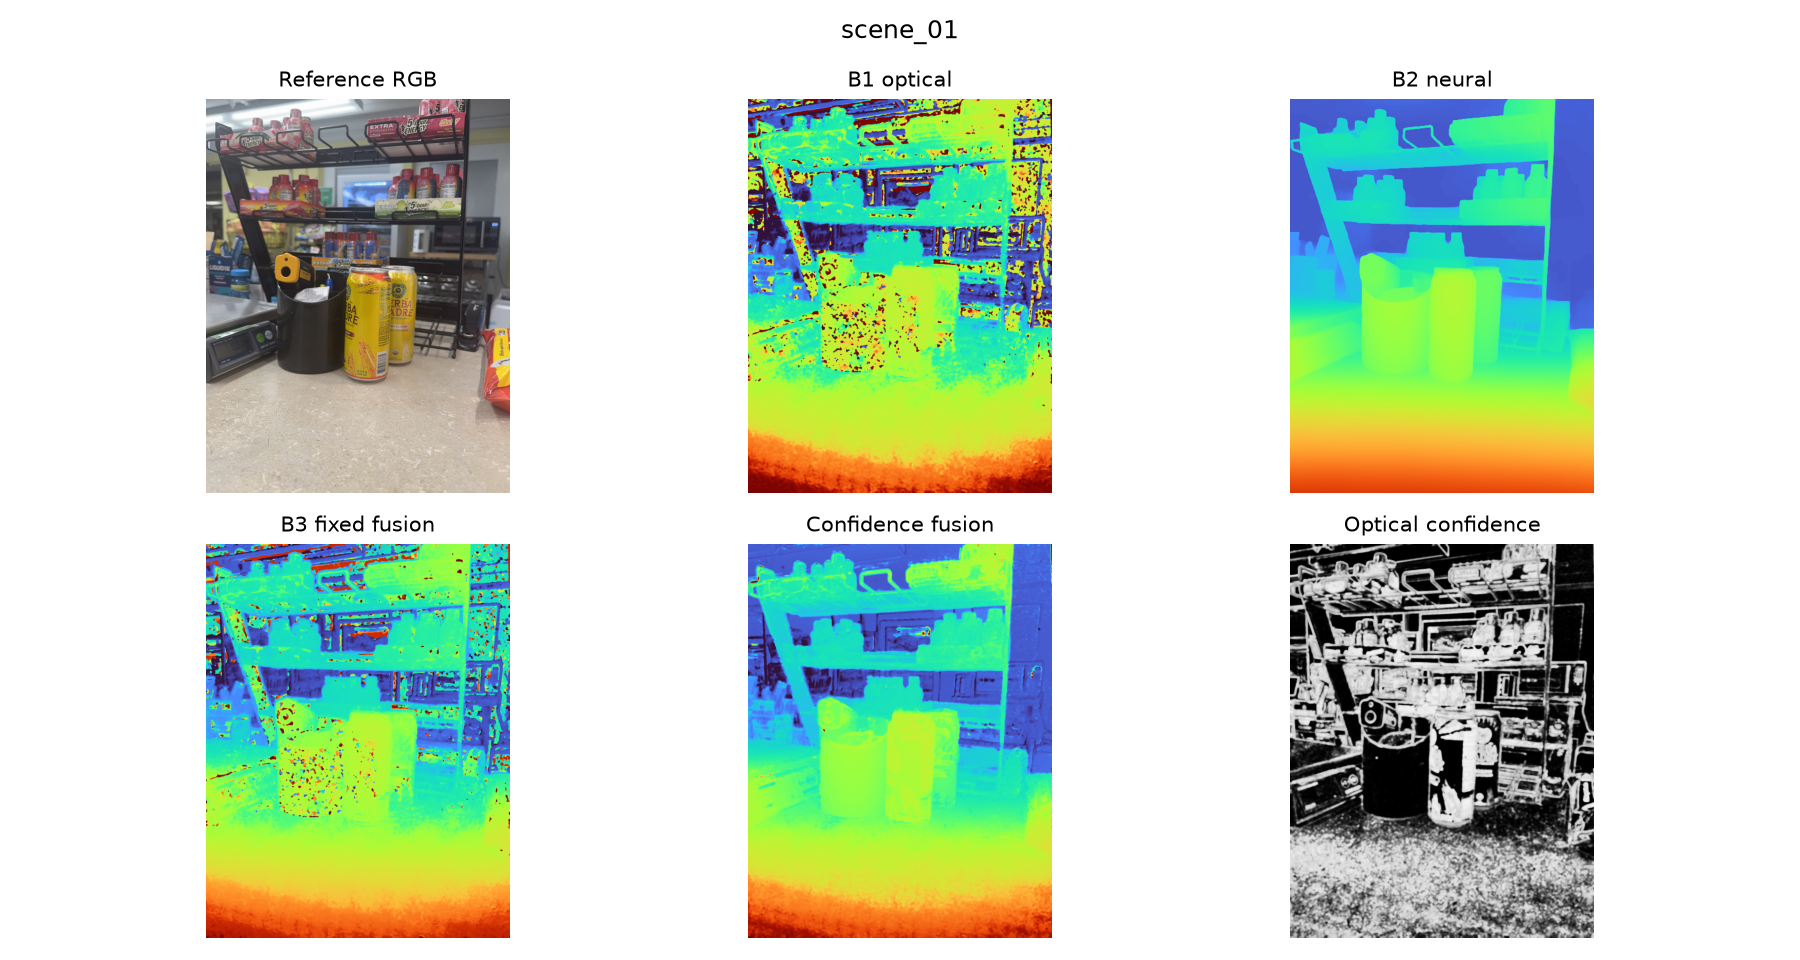
\includegraphics[width=\linewidth]{report_assets/scene_01_20261102_180021_comparison.png}
\end{center}

\noindent\textit{Figure 1. Pipeline comparison sheet for capture 180021. The associated provisional ordering evaluation gives 9/9 for every method.}\par

\begin{center}
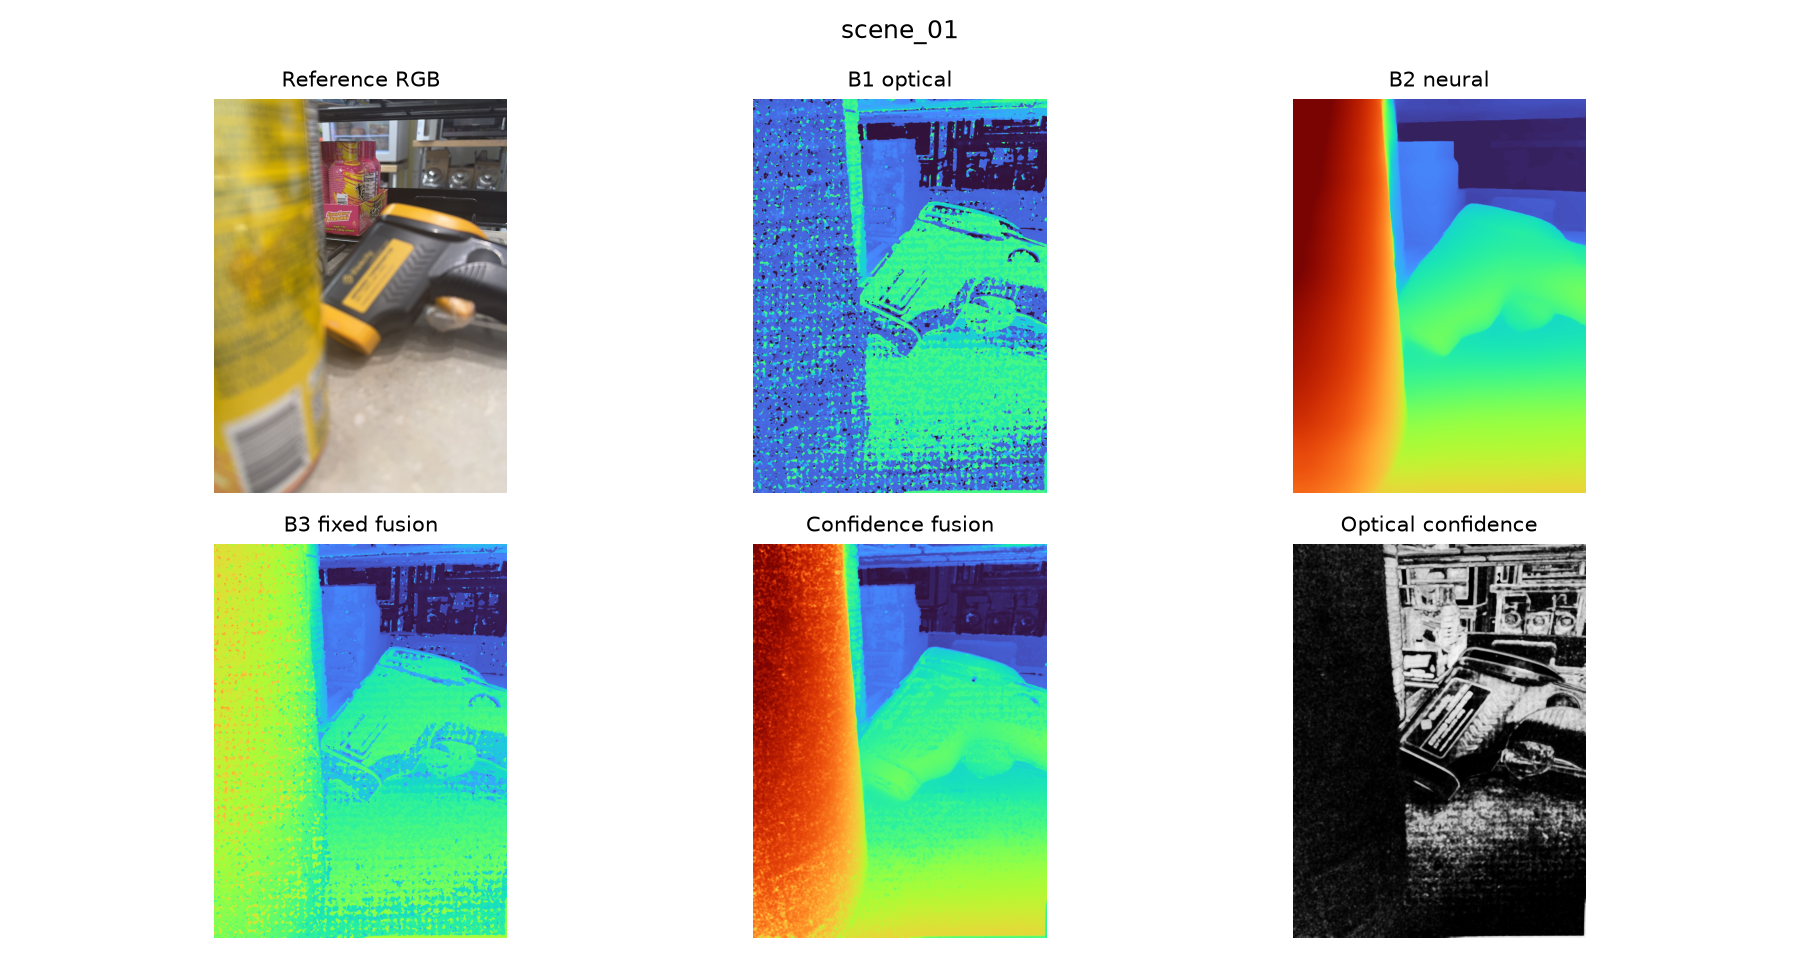
\includegraphics[width=\linewidth]{report_assets/scene_01_20261102_182153_comparison.png}
\end{center}

\noindent\textit{Figure 2. Pipeline comparison sheet for capture 182153. The nearby can is annotated as never sharp; optical ordering is 4/6 and the other three methods score 6/6 against provisional labels.}\par

These figures reside in ignored results folders. They must be bundled with any shared report or copied into a deliberate submission asset folder before export.

\section{Limitations and interpretation}

Current findings are limited by visually estimated labels, few captures, unverified repeatability, and an ordinal metric that saturates on the evaluated example. There is no dense reference depth, measured depth error, or quantitative boundary analysis. The available artifacts do not establish a separate calibration/evaluation split.

Optical coordinates require device calibration before metric interpretation. Registration errors, focus breathing, image processing, highlights, and noise can create misleading sharpness peaks. Confidence has not been calibrated against optical correctness. Per-capture neural alignment can propagate optical errors into neural and fused maps, and agreement between those maps is not independent evidence of accuracy.

The synthetic run is a software smoke test using a stand-in neural map. It is excluded from the real-capture findings and does not validate pretrained-model performance.

\section{Remaining experiments}

\begin{enumerate}
\item Replace visual distance estimates with independently measured distances and verify boxes against \path{reference_full.png}. Document uncertain orderings explicitly.
\item Inspect the nearby can's sharpness curves to explain why the optical estimate fails despite its low confidence.
\item Collect documented textured, smooth-surface, and boundary scenes, with repeated sweeps and a separate calibration set.
\item Report per-region confidence coverage and correctness, including failure cases, rather than only whole-image averages.
\item Compare fixed and confidence fusion on harder orderings; test texture-gate removal and sparse focus sampling using fixed evaluation criteria.
\item Add boundary crops, representative focus curves, capture durations, and complete processing timings.
\item Add verified primary references for depth from focus and Depth Anything V2, formatted to the course's report requirements.
\end{enumerate}

\section{Preliminary conclusion}

FocusDepth produces optical, neural, and fused relative-depth maps from exported iPhone focal stacks. One provisionally annotated capture yields nine correct region orderings for every method. A near-focus stress capture yields four of six for optical estimation and six of six for neural estimation and both fusion methods. Confidence fusion suppresses weak optical evidence but has not outperformed neural estimation or fixed fusion. The next experiments should determine whether confidence identifies optical failures and whether using it improves results on scenes where the baselines disagree.

\section{Evidence and reproduction}

The numerical tables use these local artifacts, with ordering recomputed from the saved maps by \path{scripts/analyze_ordering.py}:

\begin{itemize}
\item \path{results/scene_01_20261102_171852/metrics.json}
\item \path{results/scene_01_20261102_180021/metrics.json}
\item \path{results/scene_01_20261102_182153/metrics.json}
\item \path{data/annotations/scene_01_20261102_180021.json}
\item \path{data/annotations/scene_01_20261102_182153.json}
\end{itemize}

Method descriptions follow \path{python/run_pipeline.py}, \path{focus_depth.py}, \path{confidence.py}, \path{depth_alignment.py}, \path{fusion.py}, and \path{evaluate.py}. To recompute the latest capture with its explicit annotations (this overwrites that folder's generated outputs):

\begin{lstlisting}[basicstyle=\ttfamily\small,breaklines=true,columns=fullflexible]
python python/run_pipeline.py \
    --input data/raw/scene_01_20261102_182153 \
    --output results/scene_01_20261102_182153 \
    --annotations data/annotations/scene_01_20261102_182153.json \
    --fusion all
\end{lstlisting}

This draft records the saved state reviewed on November 2, 2026.
\end{document}
